\documentclass[preview]{standalone}

\usepackage{amsmath}
\usepackage{amssymb}
\usepackage{stellar}
\usepackage{definitions}
\usepackage{bettelini}

\begin{document}

\id{biologia-membrane}
\genpage

\section{Le membrane}

\plain{I fosfolipidi si attraggono per polarità e possono formare le seguenti composizioni}

\includesnpt[width=80\%|src=/snippet/static/membrana.png]{centered-img}

\begin{snippetdefinition}{membrana-definition}{Membrana}
    Le \textit{membrane} sono un insieme di fosfolipidi con una code e una testa idrofila.
\end{snippetdefinition}

\begin{snippet}{membrana-plasmatica-expl}
    La membrana cellulare isola fisicamente la cellula e regola lo scambio di alcune sostanze
    con l'esterno: questo fenomeno è noto come \textit{permeabilità selettiva}. La membrana cellulare
    è formata da un doppio strato fosfolipidico, dove le teste sono idrofile e quindi rivolte verso
    l'esterno, mentre le code sono idrofobe e quindi rivolte verso l'interno. La membrana è
    formata anche da proteine di membrana, che si trovano tra i fosfolipidi. In alcuni casi, queste
    proteine creano canali che permettono il passaggio di alcune sostanze attraverso la
    membrana. In altri casi, collegano l'ambiente interno con quello esterno. La membrana
    contiene anche molecole di colesterolo, che ne mantengono la struttura, rendendola della
    giusta fluidità (né troppo rigida, né troppo morbida). Attaccate alla membrana ci sono anche
    catene di circa dieci monosaccaridi, chiamate oligosaccaridi, che servono per il
    riconoscimento tra una cellula e un'altra.
    Le sostanze idrofile (steroidi, grassi, etc.) vengono trasportati nel sangue
\end{snippet}

\begin{snippetdefinition}{gradiente-concentrazione-definition}{Gradiente di concentrazione}
    Il \textit{gradiente di concentrazione} è un regolare incremento o diminuzione della concentrazione di una sostanza. Quando è presente un gradiente di concentrazione, gli ioni o le altre sostanze coinvolte tendono a muoversi spontaneamente dalla zona di concentrazione maggiore a quella di concentrazione minore.
\end{snippetdefinition}

\section{Trasporti attraverso la membrana}

\subsection{Trasporto passivo}

\begin{snippetdefinition}{trasporto-passivo-definition}{Trasporto passivo}
    Con \textit{trasporto passivo} si intende uno spostamento attraverso
    la membrana plasmatica che avviene senza consumo di energia.
    Nel trasporto passivo, le molecole si spostano secondo il gradiente di concentrazione,
    ovvero da dove sono maggiormente concentrate a dove lo sono meno.
\end{snippetdefinition}

\includesnpt[width=50\%|src=/snippet/static/trasporto-passivo.png]{centered-img}

\subsection{Diffusione}

\begin{snippetdefinition}{diffusione-definition}{Diffusione}
    La \textit{diffusione} è il fenomeno per il quale le particelle tendono a distribuirsi in modo
    uniforme nello spazio disponibile.
\end{snippetdefinition}

\begin{snippetdefinition}{diffusione-semplice-definition}{Diffusione semplice}
    La \textit{diffusione semplice} è una tipologia di trasporto passivo in cui molecole di piccole dimensioni, apolari o polari
    non cariche possono attraversare il doppio stato fosfolipidico della membrana.
\end{snippetdefinition}

\begin{snippetexample}{diffusione-semplice-example}{Diffusione semplice}
    O\({}_2\), H\({}_2\), benzene, HO\({}_2\), glicerolo, CO\({}_2\).
\end{snippetexample}

\begin{snippetdefinition}{diffusione-facilitata-definition}{Diffusione facilitata}
    La \textit{diffusione facilitata} è una tipologia di trasporto passivo che permette a determinate molecole di attraversare la
    membrana cellulare mediante proteine di trasporto, che si trovano nello strato fosfolipidico.
    Le molecole che utilizzano questo tipo di trasporto sono molecole grandi, polari o ioni.
\end{snippetdefinition}

\begin{snippetexample}{diffusione-facilitata-example}{Diffusione facilitata}
    glucosio, H\({}^+\), Na\({}^+\), K\({}^+\), Mg\({}_2^+\), Ca\({}_2^+\), Cl\({}^-\).
\end{snippetexample}

\includesnpt[width=50\%|src=/snippet/static/diffusione-facilitata.png]{centered-img}

\subsection{Proteine di membrana}

\begin{snippet}{protiene-trasporto-scopo}
    Per consentire la diffusione facilitata, le più
    comuni proteine di trasporto agiscono come un canale che alcune molecole o ioni
    attraversano superando la membrana. La proteina di trasporto è specifica per
    la sostanza di cui facilita il passaggio. Maggiore
    è il numero di proteine di trasporto per un particolare soluto, più rapida è la sua diffusione
    attraverso la membrana.
\end{snippet}

\begin{snippetdefinition}{proteina-trasporto-definition}{Proteina di trasporto}
    Una \textit{proteina di trasporto} (canale) è una proteine di membrana che forma un tunnel sempre aperto.
    Ogni canale non è direzionale ed ogni canale è specifico per un certo soluto.
\end{snippetdefinition}

\includesnpt[width=80\%|src=/snippet/static/proteine-mem.png]{centered-img}

\begin{snippetdefinition}{trasportatore-definition}{Trasportatore}
    Un \textit{trasportatore} è una proteina che sposta una sostanza contro il gradiente.
\end{snippetdefinition}

\begin{snippet}{e9287974-8fcf-4bdd-ab3d-d647549dad77}
    Ogni tipo di trasportatore è specifico ad un tipo di sostanza.
    Il trasportatore sposta quindi una sostanza da dove ce n'è poca a dove ce n'è tanta (mediante energia).
\end{snippet}

\begin{snippetdefinition}{ricettore-definition}{Ricettore}
    Un \textit{ricettore} è una proteina che comunica dei messaggi alla cellula.
\end{snippetdefinition}

\begin{snippetexample}{ricettore-example}{Ricettori}
    Un ricettore potrebbe per esempio comunicare il segnale della presenza di un agente patogeno.
\end{snippetexample}

\subsection{Trasporto attivo}

\begin{snippetdefinition}{trasporto-attivo-definition}{Trasporto attivo}
    Il \textit{trasporto attivo} è un processo che consiste nel trasporto di sostanze attraverso la membrana contro il gradiente
    di concentrazione, cioè dalla parte in cui sono meno concentrate a quella in cui la loro
    concentrazione è maggiore. Questo processo richiede il consumo di energia, che proviene
    dalle molecole di ATP. Il trasporto attivo permette a una cellula di mantenere la
    concentrazione interna di alcune piccole molecole diversa da quella dell'ambiente
    circostante.
\end{snippetdefinition}

\includesnpt[width=30\%|src=/snippet/static/trasporto-attivo.png]{centered-img}

\begin{snippetdefinition}{trasporto-attivo-primario-definition}{Trasporto attivo primario}
    Il \textit{trasporto attivo primario} è un trasporto grazie ad un trasportatore e all'ATP.
\end{snippetdefinition}

\begin{snippetdefinition}{trasporto-secondario-definition}{Trasporto attivo secondario}
    Il \textit{trasporto attivo secondario} sfrutta il trasporto attivo primario
    senza costo.
    Questo tipo di trasporto di divide nelle seguenti categorie.
    \begin{itemize}
        \item \textit{uniporto:} consente il passaggio di un solo ione o molecola in un'unica direzione;
        \item \textit{antiporto:} consente il passaggio contemporaneo ma in direzioni opposte di due ioni e/o molecole differenti;
        \item \textit{simporto:} consente il passaggio contemporaneo ma nella stessa direzione di due ioni e/o molecole differenti.
    \end{itemize}
\end{snippetdefinition}

\begin{snippet}{uniporto-antiporto-simporto-illustration}
    \begin{figure}[h!]
        \begin{minipage}{0.3\textwidth}
          \centering
          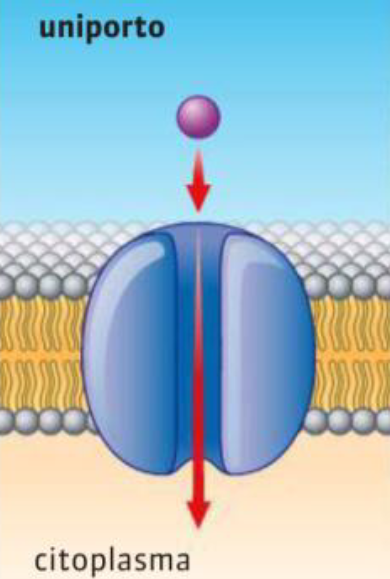
\includegraphics[width=\linewidth]{resources/uniporto.png}
        \end{minipage}%
        \hfill
        \begin{minipage}{0.3\textwidth}
          \centering
          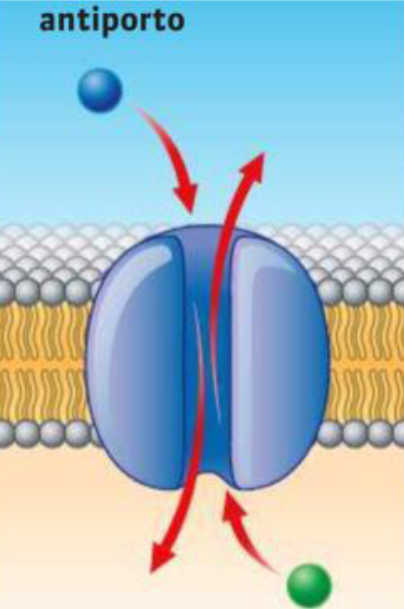
\includegraphics[width=\linewidth]{resources/antiporto.png}
        \end{minipage}%
        \hfill
        \begin{minipage}{0.3\textwidth}
          \centering
          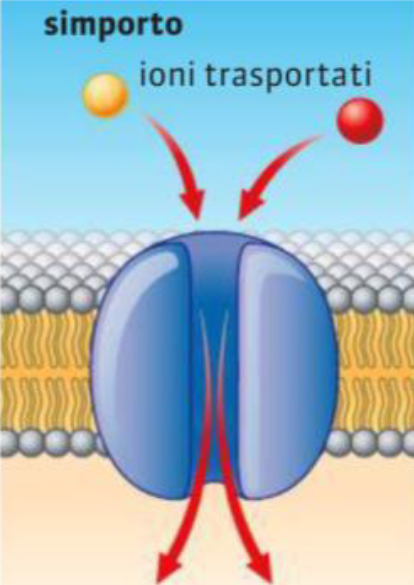
\includegraphics[width=\linewidth]{resources/simporto.png}
        \end{minipage}
    \end{figure}
\end{snippet}

\subsection{Trasporto vescicolare}

\begin{snippet}{3d67130a-ec53-469e-ae6b-c28f2e1d40f5}
    Quando le molecole sono troppo grandi (es. proteine intere) per passare per un canale, possono essere trasportate 
    mediante una \textit{vescicola di trasporto}. Il processo di entrata si chiama \textit{endocitosi},
    mediante quello di uscita si chiama \textit{esocitosi}. 
    In questa illustrazione il colore blu rappresenta il contenuto di un organello.
\end{snippet}

\includesnpt[src=https://www.youtube.com/embed/uYpNUw7vPO4]{yt-embed}

\subsection{La pompa sodio-potassio}

\begin{snippet}{pompa-sodio-potassio-expl}
    Rispetto all'ambiente esterno, una cellula animale ha al proprio interno una concentrazione
    di ioni potassio (K\({}^+\)) superiore e una concentrazione di ioni sodio (Na\({}^+\)) inferiore. Da questa
    differenza di concentrazione dipendono molti processi cellulari, tra cui la generazione e la
    trasmissione degli impulsi nervosi. Una proteina di trasporto chiamata pompa sodio potassio
    aiuta le cellule a mantenere questi gradienti muovendo gli ioni Na\({}^+\) e K\({}^+\) attraverso la
    membrana plasmatica. In un processo chiamato \textit{fosforilazione}, l'ATP cede direttamente alla
    pompa sodio-potassio uno dei tre gruppi fosfato di cui è composto, insieme all'energia
    necessaria al trasporto attivo.
\end{snippet}

\includesnpt[width=80\%|src=/snippet/static/pompa-sodio-potassio.png]{centered-img}

\subsection{Schema riassuntivo}

% https://tikzcd.yichuanshen.de/#N4Igdg9gJgpgziAXAbVABwnAlgFyxMJZAFgBoBGAXVJADcBDAGwFcYkQAdDnGADxwBGAM2ABBHHloQAviGml0mXPkIoAbBWp0mrdlx79hwAAr042KbPmLseAkQDMpAExaGLNok7c+OEwCcsAFt6QIgAAgAKUQAVYwBKKwUQDFsVIgBWFzcdT28DPwBlGABjAihQ-CSbZXsUMgccjz0ffmAAVTAsDH8cGTlk1NrVZCzGmnddL31fYELgnr7qlKU7EY1x7Wbp1r9RMDxF-usVtLrkDWImqZABmrXM0iuJ3PY70+GiMmetm-ehh4oAAcmhe23yswAIlghEJmNgCDBlgD0igAJzZME3GZtYpBNCMLAlJH-Vao5AAdkxvzyOL8ADF6CUsIScPQ2ciyecqZtJrTdsASvQwEwsJyziMMbzXjsCsAgjAggJ-ML6OLPvVSAAGa78gpGGIquCLMWkiVEZygmktfUiABq8GZZUYoRJJxR53I2t1NtmAFEwFAIMy+th1YDkF7XFi9f64MHcEpw+StVa+b62gBxFWBrDhND+CA8LBgN2DLkjL3S8F03DAP1wAB04Wk4TpwEzLBwxCsWhgUAA5vAiKAhIWgkhUyA+khnCcxxAJ4gpzPEA55+OkE5pxAkD3kgul9vVxkN4utzRV2oz0uNDukFSQAIYIGkABaBxam8Py+7xB359X0QD8vwPTdECye9EBBEBCVLdh40JKAQBoAALGB6GQxAwGYRhGEvegWXYSB4JoQCsKnOBUJhHAkHIb9EDIKC0QY8gVz-ch6LA89EDY386Lnbil3IS0oPIdchLor0xP3UdwPISDVynF1n0YYwK3YQIB1Q2iYwzPwAGECBwQtwmzTCsBfHhlkPOjFI4siXywz89NlWZjBgfwzJVKBLIOEkaBUmA1I0rwtJ095bN4+y6IApz30-Vi71XcgKSS-jeKBViMTEu84LyCoqP7FDp0Ixh2DZIi0IwrDpwAdwgdDMIQBjnHY2LHKAkDApLAqix4ZDAvoVT1PNLwS2wWASvTNzDBENAzAsY5JN4jK2IY48-1EmaITaOAx2YCQ1RK-L2CDCRioYmLoM6iiaComj33oyhpCAA

\includesnpt[width=80\%|src=/snippet/static/schema.png]{centered-img}

\end{document}